\clearpage
\begin{flushright}
	\textit{Лекция №8}
	\textit{2015.10.06}
\end{flushright}

\subsubsection{Aссоциативное отображение}

Предполагает наличие в системе специального вида памяти – ассоциативной. Ассоциативная память – дорогая, регистровая, катастрофически возрастает кол-во соединений. Позволяет произвести выборку информации за один такт. Параллельное сравнение ключа с другими ключами.

\begin{figure}[H]
    \centering
    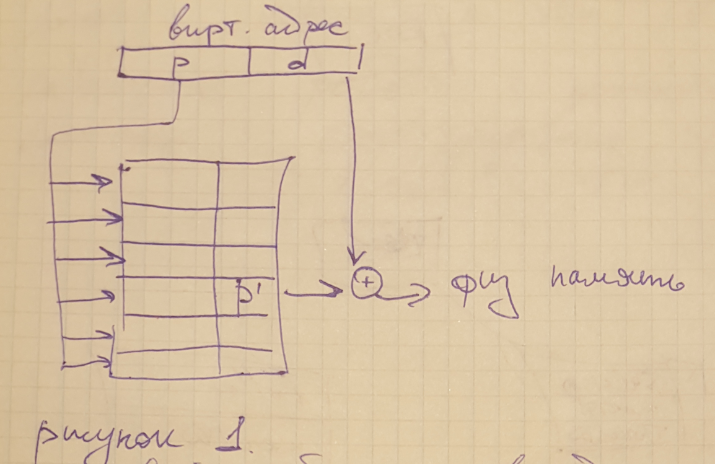
\includegraphics[width=\textwidth]{pic/1.png}
    \caption{pic}
\end{figure}

\subsubsection{Ассоциативное – прямое отображение}
В процессоре есть регистр базового адреса таблицы страниц. В нем содержится начальный адрес таблицы страниц в оперативной памяти. Страница сначала ищется в ассоциативном кэше. Если в кэше нет, то происходит обращение к физической памяти. Замещение происходит тех страниц, к котором обращение было давно. 

\begin{figure}[H]
    \centering
    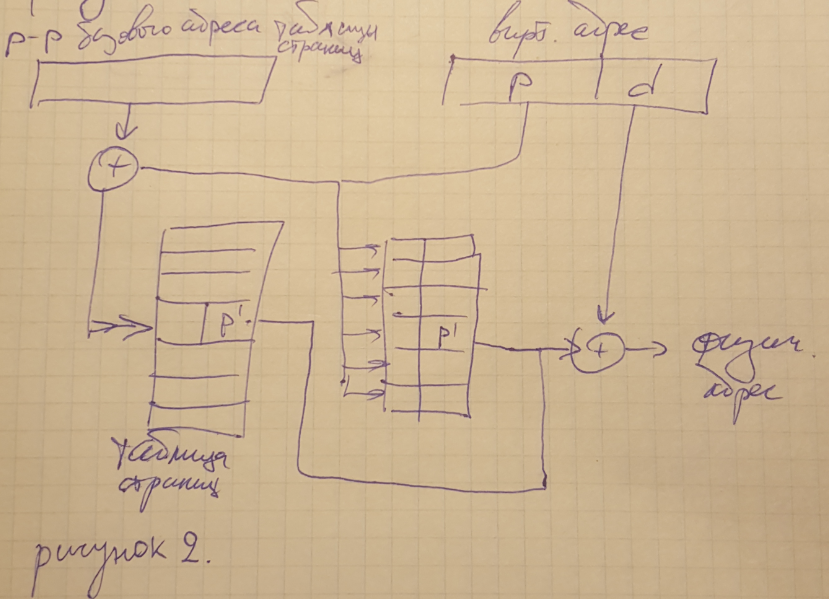
\includegraphics[width=\textwidth]{pic/2.png}
    \caption{pic}
\end{figure}

В процессорах Intel есть кэш TLB. Не полностью ассоциативный кэш, а частично ассоциативный. Используя алгоритм LRU, имея ассоциативный буфер 8 – 16 строк позволяет достичь порядка ~90\% характеристик полностью ассоциативного кэша, в который мы могли бы загрузить всю таблицу страниц.
В системе столько таблиц, сколько процессов. При смене процесса актуальность кэша = 0. Таблицы страниц должны находиться в оперативной памяти. Эти таблицы пожирают ОЗУ. IBM была предложена двух уровневая организация таблиц страниц. Вводится понятие гиперстраницы. Виртуальный адрес делится на 3 части. Сохраняется стремление использовать ассоциативный буфер. Адресное пространство процесса делится на гиперстраницы, которые делятся на страницы. В результате таблиц страниц будет много, а таблица гиперстраниц – одна. Из таблицы гиперстраниц получаем базовый адрес таблицы страниц. P – смещение таблицы страниц. Если необходимой страницы нет в кэше, то обращаемся к ??? и получаем адрес страницы физической памяти, который можем использовать для ??? линейного адреса. Мы можем выгружать те таблицы страниц, которые в данный момент не используются ( к которым не было обращения).

\begin{figure}[H]
    \centering
    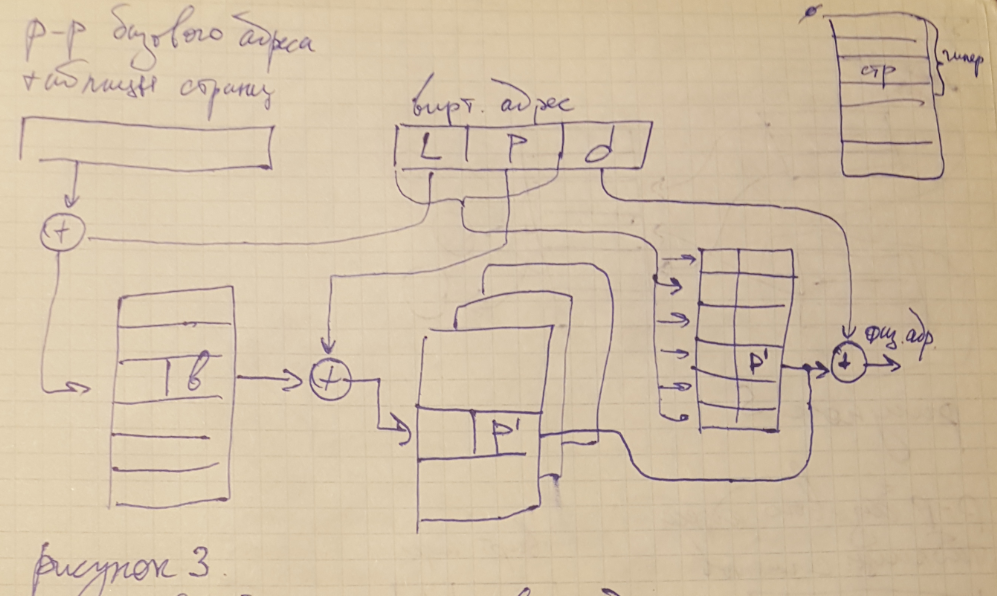
\includegraphics[width=\textwidth]{pic/3.png}
    \caption{pic}
\end{figure}

Copy-on-write решает проблемы с коллективным доступом. Страницу мы должны разделять. Разделение выполняется по принципу Copy-on-write. Если процесс захочет записать в страницу, то в его адресном пространстве будет создана копия страницы. Основная претензия к страничному ??? была снята. Intel поддерживает страницами по запросам и сегментами по запросам. Наличие регистра CR3 доказывает наличие независимого табличного преобразования.

\subsection{Схема преобразования сегментами по запросам}

Страница – физическое деление памяти. Сегмент – логическое деление памяти. Размер сегмента определяется размером программного кода. При сегментном преобразование необходимо проверять, не вышел ли процесс за собственное адресное пространство. Процесс имеет таблицу сегментов. Виртуальный адрес делится на 2 части: сегмент, смещение. В дескрипторе сегмента присутствует размер сегмента, при формировании адреса выполняется проверка.

\begin{figure}[H]
    \centering
    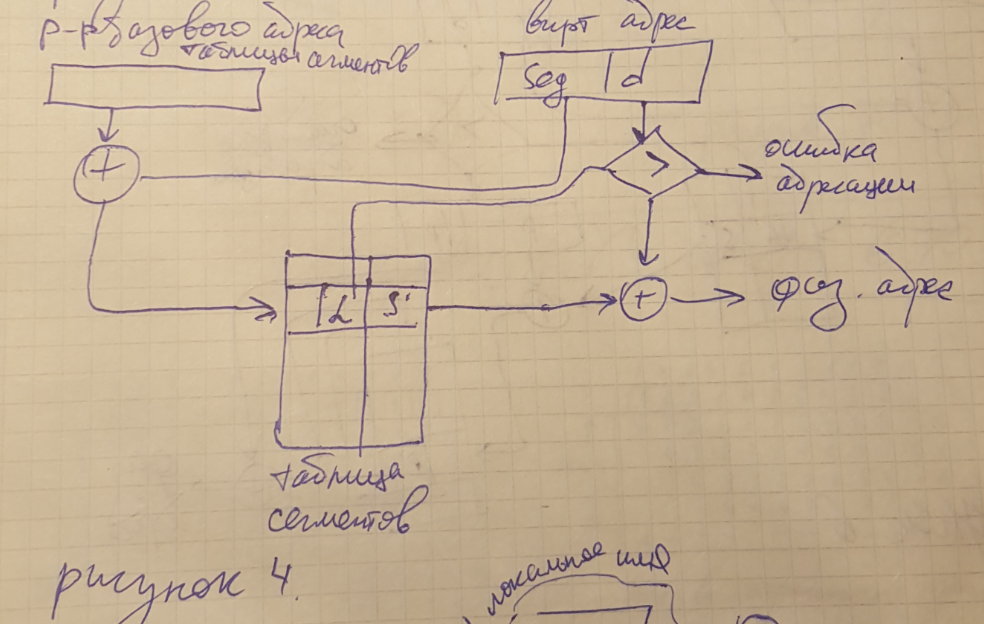
\includegraphics[width=\textwidth]{pic/4.png}
    \caption{pic}
\end{figure}

Организация ???:
\begin{enumerate}
    \item единая таблица. У сегментов в системе есть глобальное имя.
    \item локальные таблицы. ???. Сегмент имеет локальное имя.
    \item локальная таблица + глобальная. У каждого процесса есть возможность работать по его локальному имени и то же время есть глобальная таблица, описывающая сегменты памяти и обращения к сегментам памяти выполняется по глобальному имени.
\end{enumerate} 

\begin{figure}[H]
    \centering
    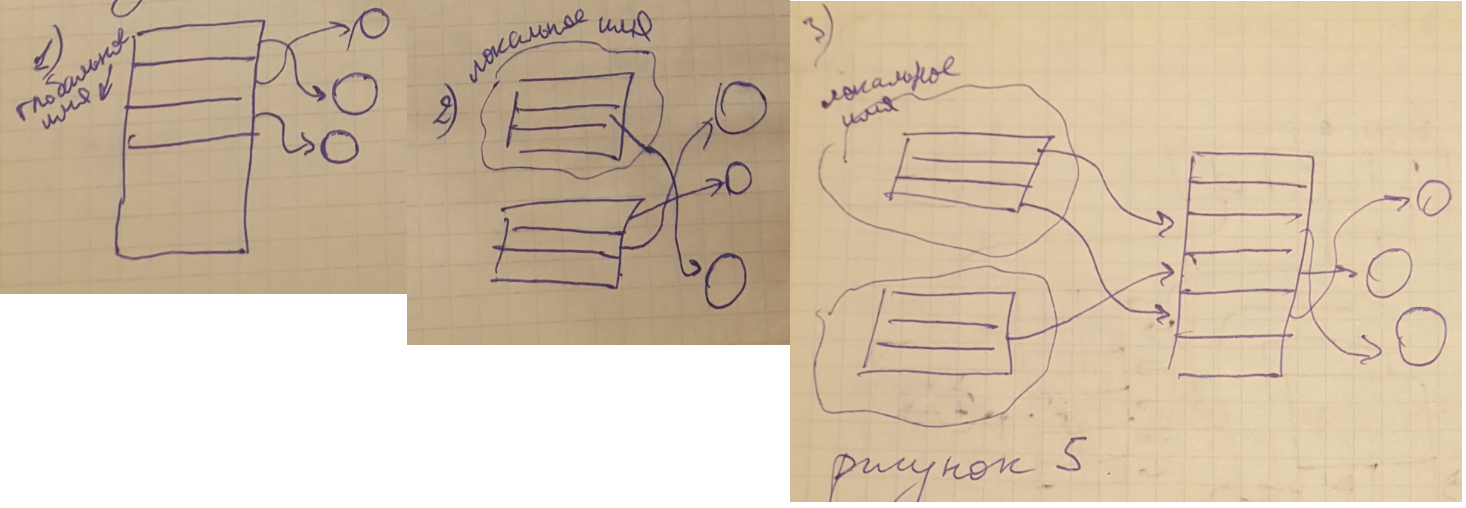
\includegraphics[width=\textwidth]{pic/5.png}
    \caption{pic}
\end{figure}

\subsection{Управление памяти сегментами, поделенными на страницы}

В выделении памяти разделами переменного размера были проблемы с фрагментацией памяти. Наши сегменты – перемещаемые, но надо поменять физические базовые адреса. Отредактировать все таблицы или глобальную таблицу.  Большой объем работ, связанных с объединением свободной памяти. Цена вопроса? Намучавшийся с сегментами, люди придумали управление памяти сегментами, поделенными на страницы. Адресное пространство процесса делится на сегменты, но размер сегмента должен быть кратен размеру страницы. Есть таблицы сегментов, но в ней будет находится базовый адрес таблицы страницы сегмента. Если программа поделена на несколько сегментов, то будет несколько таблицы страниц. Смещение делится на 2 части: страницу и смещение в странице. В таблице сегментов находится базовый адрес таблицы страниц этого сегмента.

\begin{figure}[H]
    \centering
    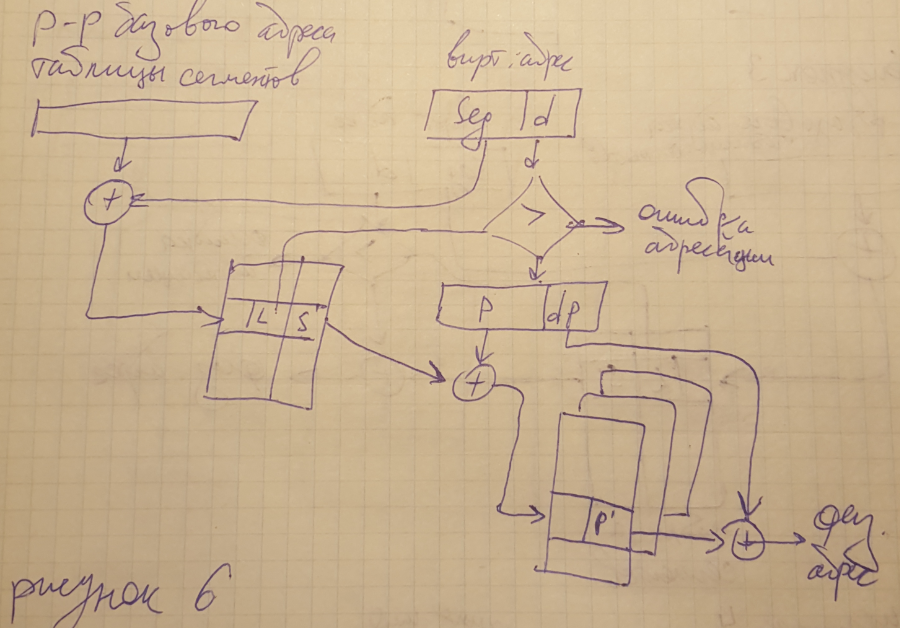
\includegraphics[width=\textwidth]{pic/6.png}
    \caption{pic}
\end{figure}

\begin{figure}[H]
    \centering
    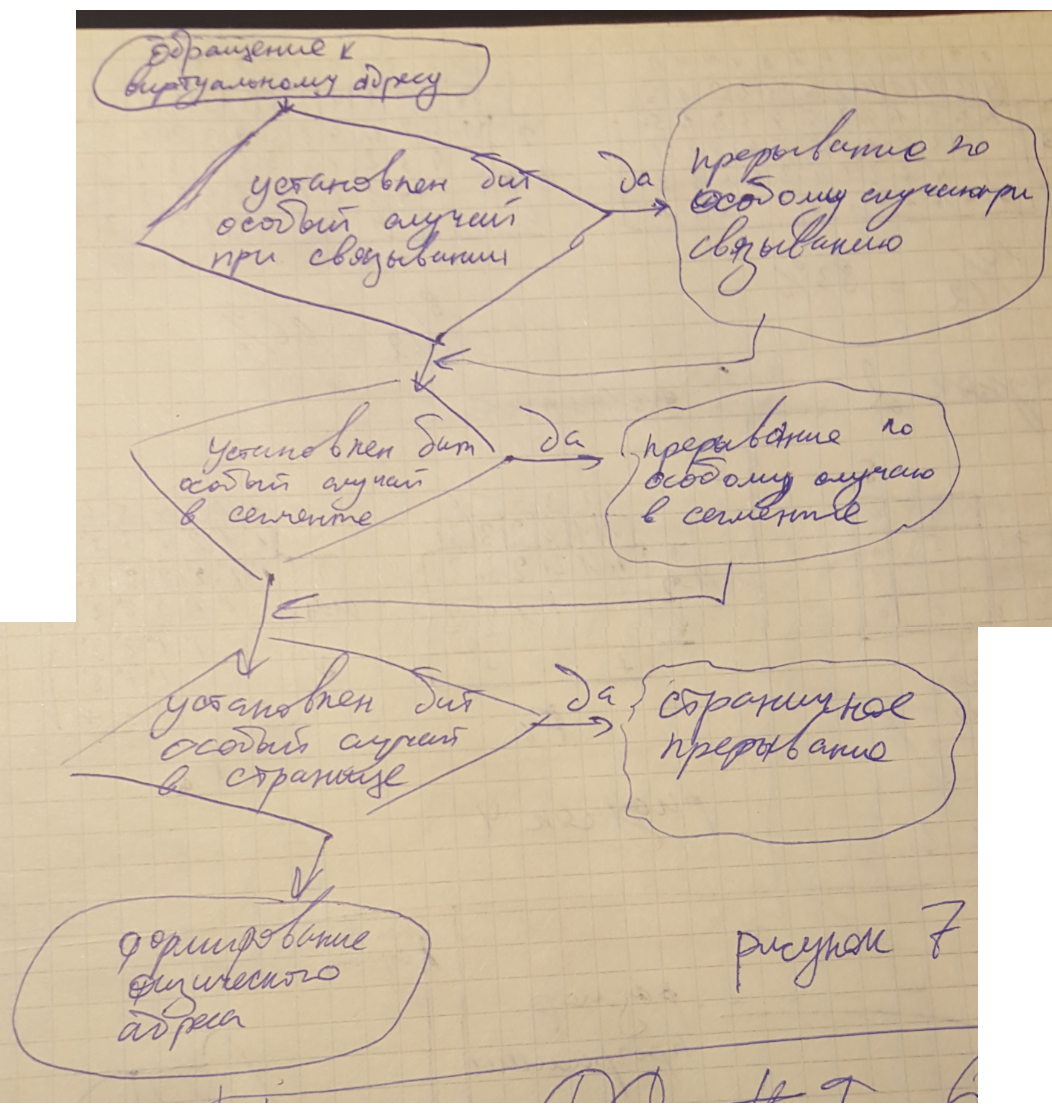
\includegraphics[width=\textwidth]{pic/7.png}
    \caption{pic}
\end{figure}

Речь идет об отложенном связывании (linking). Программа поделена на сегменты, сегмент линкуется только когда к нему происходит обращение и выполняется в процессе выполнения программы.  Прерывание по особому случаю при связывании: появление в таблице сегментов данного процесса дескриптора данного сегмента. Для данного сегмента будет создана таблица страниц и это будет сделано по прерыванию по особому случаю в сегменте. И уже по страничному прерыванию, использую таблицу страниц сегмента менеджер памяти сможет загрузить необходимую страницу в физическую память. В результате получим адрес начала ??? физической памяти и сложив со смещением получим линейный адрес. Свопинг заменяем пейджингом. Остается физическое деление памяти (сегменты делятся на страницы). При использовании copy-on-write преимущество данной схемы в ноль. 

